% Historical TCP evaluation, superseded by the NCCL experiment; not compiled.
\subsection{Heterogeneous two-host execution}
\label{sec:two-host}
The next experiment uses both available GPUs: the RTX 5070 Ti Linux host and
an RTX 4070 Ti SUPER (16 GiB) under Ubuntu/WSL on a second Windows host. They
communicate over the private network using TCP host staging. Both retain their
existing service workloads; about 3 GiB and 10--11 GiB of GPU memory were already
occupied. This is not a same-host NVLink/PCIe experiment or a dedicated cluster.
Both rank records contain matching hashes for every Tiga Python source and both
compiler executables. Environment and driver versions are retained per rank.

The graph has 16 edges per row and 16 FP32 features. Destination ownership is
split equally. Three quarters of the rows gather within their owner's half;
every fourth row gathers 16 neighbors from the other half. Overlapping remote
neighborhoods make the required ghost set large: boundary-row fraction alone
is not the exchanged-byte fraction. The sizes are 8,192, 32,768 and 131,072 nodes.
Each GPU also runs the complete graph alone with identical values and semantics.
This is strong scaling of one fixed graph, not doubling the graph with the ranks.
Topology is replicated for setup on both hosts and its partition maps are cached;
runtime source fields contain only owned rows before halo exchange. This is not
evidence that the topology itself was distributed beyond one device's capacity.

Each configuration has three warmups and ten measured calls with changed input
scales. Every output is checked against an independent NumPy construction of
the global result. Timings are synchronized host-wall intervals through output
completion, excluding graph/input creation, an inter-rank control barrier and
oracle checking. The distributed critical path is the maximum of the paired
rank durations for each round; it is not the average of two ranks. The methods
run in a fixed order, so drift and other host workloads remain confounders.
These native-input host-wall measurements are not interchangeable with the
earlier ordinary-Torch CUDA-event measurements.

\begin{figure}[htbp]
\centering
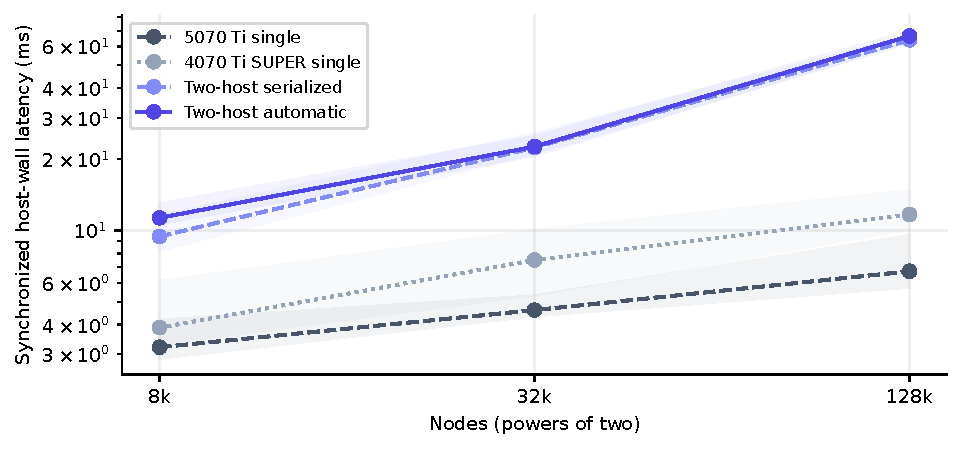
\includegraphics[width=.94\linewidth]{figures/two-host-latency.pdf}
\caption{Real two-host TCP scaling versus each GPU running the complete graph.
Lines are medians; bands show sample minima and maxima. Lower is better.
This configuration provides no multi-GPU speedup.}
\label{fig:two-host}
\end{figure}

At 131,072 nodes, the 5070 Ti and 4070 Ti SUPER single-GPU medians are 6.72 and
11.68 ms. Two-host serialized execution takes 64.00 ms and the automatic path
66.46 ms on the paired critical-path definition. At the smallest size the
automatic path is also slower than serialization (11.31 versus 9.44 ms).
Correctness and execution on two devices therefore do not establish useful
scaling. Automatically creating interior/boundary work is not a successful
cost model for deciding when its extra launches and assembly pay off.

\begin{figure}[htbp]
\centering
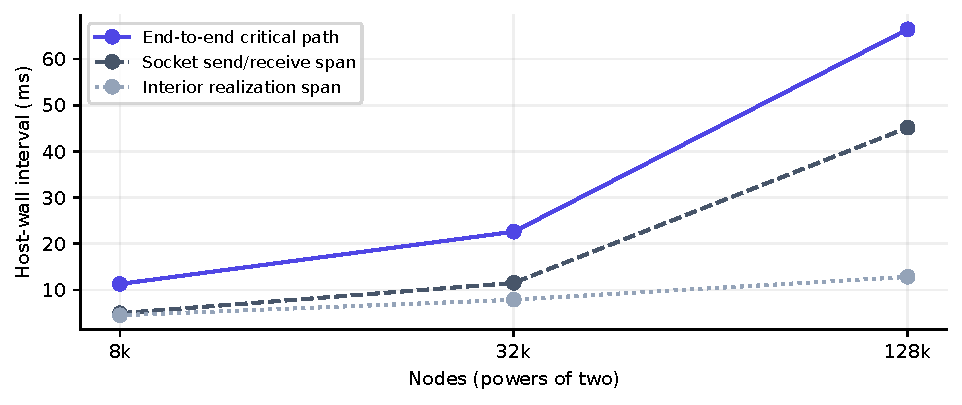
\includegraphics[width=.94\linewidth]{figures/two-host-components.pdf}
\caption{Host intervals in the automatic two-host run. Socket span covers the
first send/receive entry through the last return, including waits; it excludes
some packing, device copies and assembly. Interior realization includes host
submission. These intervals can overlap and must not be stacked or added as
exclusive components; they are not GPU-profiler measurements.}
\end{figure}

The raw records include sent/received payload bytes and per-rank interval traces.
The observed costs motivate reducing host staging, Python packing and repeated
assembly, and evaluating transport-aware scheduling. They do not prove that a
different transport or partition would deliver a particular speedup.

The NCCL configuration connects the two hosts through an isolated WireGuard
interface with bidirectional private addresses and MTU 1200. This fits the
WSL host's 1280-byte outer-interface MTU without changing the default route.

Both machines then passed a checked bidirectional 1 MiB exchange with the same
NCCL 2.28.9 library hash. A separate eight-node ring graph also passed forward
and source-VJP checks on both GPUs, in serialized and automatic schedules and
with changed inputs. The automatic trace reports two interior and two boundary
rows per rank; doubled input scale doubles the expected gradient from 3 to 6.
The runtime uses NCCL's device-buffer interface, but NCCL selects its Socket
network plugin over the encrypted tunnel, not GPUDirect RDMA. These are
correctness gates, not a bandwidth benchmark, scaling curve or device-profiler
proof of useful overlap. Earlier TCP timing curves are unchanged. Commands,
library/source hashes and both ranks' results accompany the report in
\code{data/runtime/}.
\FloatBarrier

% Original capacity discussion; data reused in evaluation-questions.tex. Not compiled.
\subsection{Billion-edge execution on a 16 GiB GPU}
\label{sec:gpu-paging}
The capacity experiment evaluates a graph whose full resident working set
exceeds the GPU's physical memory. The largest configuration contains exactly
one billion directed edges, 62.5 million nodes and 32 FP32 source features.
Every destination gathers its next 16 neighbors on a periodic ring and computes
their mean. The explicit CSR uses 64-bit indices; all edges are stored and
traversed, without replacing message passing by an analytic stencil kernel.
This regular-local topology isolates capacity and streaming costs; it does not
represent random power-law gathers.

The CSR occupies 8.50 GB and the source and output fields occupy 8.00 GB each.
Their combined resident lower bound is 24.50 GB (22.82 GiB), before scratch
buffers or compiler allocations. Thus full residency exceeds a 16 GiB device
even without other services. This is a lower-bound capacity comparison, not
an observed out-of-memory timing and not a claim that every alternative sparse
implementation requires these bytes: narrower indices or compressed relations
can change the footprint. Even with 32-bit CSR indices, the same source and
output fields give an 18.86 GiB lower bound, still above device capacity.

The fixture writer emits bounded chunks into the versioned CSR store and
records hashes of all three payloads. The public loader opens metadata-only
field handles. Execution streams 65,536 destination rows at a time, gathers
source values into host staging, copies the page to CUDA, and lowers FP32 CSR
sum to a bounded per-row reduction. Completed pages are written into the final
resident output through a single reusable-size host payload. The 7.45 GiB
output must fit device memory; the full input need not be resident there.
Each worker has a 12 GiB native-allocation safety budget, reduced if needed to
leave 512 MiB of currently free device memory uncommitted. Existing services
occupy about 3 GiB. The capacity comparison uses the physical device size,
not this software budget.

Each trial runs one forward in a fresh process. Time includes JIT lookup or
compilation, page reads, host/device copies, computation and output assembly.
Fixture construction, process startup, graph-handle loading and the independent
oracle are recorded separately. Every output element is checked in bounded
chunks against a modular-arithmetic oracle; the oracle alone exploits the
ring's regularity. Three graph sizes distinguish growth with edge count from
fixed setup costs. Device-wide memory is sampled once per second, separately
from native allocation accounting and process peak RSS. Other GPU services
remain active, and the OS page cache is not forcibly cleared.

\begin{figure}[htbp]
\centering
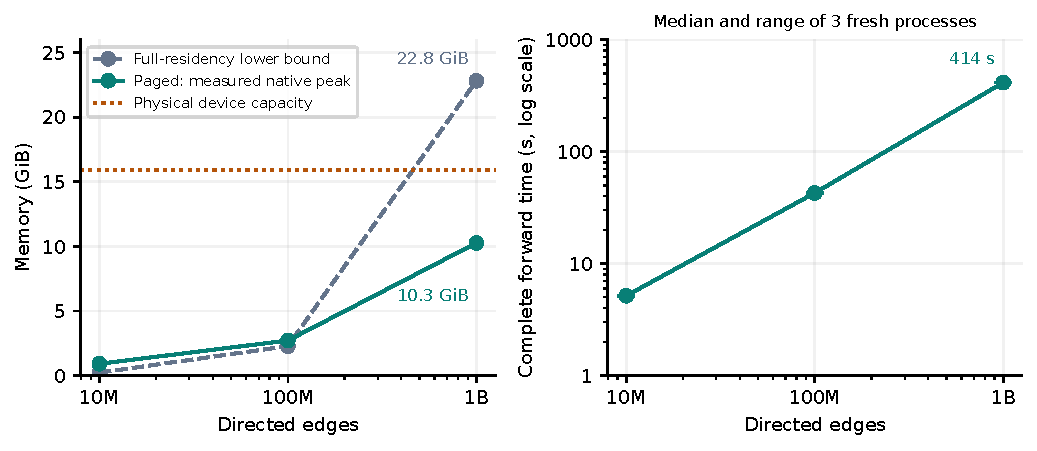
\includegraphics[width=\linewidth]{figures/billion-capacity.pdf}
\caption{One billion explicit edges on a single RTX 5070 Ti. Left: measured
native allocation peak versus the calculated full-residency lower bound, not
an executed resident baseline. Right: median and range of three complete
forward calls in fresh processes, including host staging and output assembly.}
\label{fig:billion}
\end{figure}
All nine trials complete with zero elementwise error. At one billion edges, the median forward takes 414.25 s (range 411.36--415.61 s). The maximum native GPU allocation peak across trials is 10.27 GiB, including the 7.45 GiB output; forward process peak RSS is 8.83 GiB. The maximum sampled whole-device usage is 13.25 GiB, including existing services and runtime pools; one-second sampling is not an exact physical peak. Each trial checks all two billion FP32 output values outside the forward timing interval.

\FloatBarrier

This evaluates forward capacity, not a speedup over an executable billion-edge
resident baseline, training throughput, GPUDirect Storage or cold-NVMe bandwidth.
The workload fits host RAM, and the output remains on the GPU. Recurrent
execution under a controlled smaller budget is evaluated separately in
Appendix~\ref{app:recurrent}; it is not extrapolated to billion-edge recurrence.
\FloatBarrier

